\documentclass{article}
\usepackage{booktabs} 
\usepackage{geometry}
\usepackage{longtable}
\usepackage[dvipsnames,table]{xcolor}
\usepackage{fancyhdr}
\usepackage{xcolor}
\usepackage{graphicx}
\usepackage{hyperref}
\usepackage{float}
\usepackage{listings}
\usepackage{amssymb}
\usepackage{amsmath}
\usepackage{enumitem}
\usepackage{parskip}
\usepackage[table]{xcolor}
\usepackage{longtable}
\usepackage{colortbl}
\usepackage[dvipsnames,table]{xcolor}
\usepackage{caption}       % For \captionof
\usepackage{tabularx}      % For tables with adjustable-width columns
\usepackage{circuitikz}    % For circuit diagrams
\definecolor{dark-gray}{HTML}{585858}  % Dark gray


% Choose paper size
\geometry{letterpaper, top=25.4mm, bottom=25.4mm, left=25.4mm, right=25.4mm}
%\geometry{a4paper, top=25.4mm, bottom=25.4mm, left=25.4mm, right=25.4mm}

\color{black}
\fancyhf{}
\renewcommand{\headrulewidth}{1pt}
\renewcommand{\footrulewidth}{1pt}

% Define standard IPF color palette
\definecolor{soft-sky-blue}{HTML}{B7DAEB}
\definecolor{orange}{HTML}{FF6633}
\definecolor{cool-grey}{HTML}{91A1B0}
\definecolor{black}{HTML}{000000}
\definecolor{space-blue}{HTML}{003366}
\definecolor{pigeon-blue}{HTML}{5F8396}
\definecolor{sage-green}{HTML}{95A077}
\definecolor{fire-yellow}{HTML}{F9A651}
\definecolor{apple-red}{HTML}{CC4200}
\definecolor{crockadile-green}{HTML}{718944}
\definecolor{slate-grey}{HTML}{607587}
\definecolor{fog-grey}{HTML}{E5E6E9}

% Define certification colors
\definecolor{cert-level-0}{HTML}{CC4200} % apple-red
\definecolor{cert-level-1}{HTML}{FF6633} % orange
\definecolor{cert-level-2}{HTML}{F9A651} % fire-yellow
\definecolor{cert-level-3}{HTML}{B7DAEB} % soft-sky-blue
\definecolor{cert-level-4}{HTML}{5F8396} % pigeon-blue
\definecolor{cert-level-5}{HTML}{718944} % sage-green

\hypersetup{hidelinks}
\pagestyle{fancy}
\pagenumbering{arabic}

\title{

\includegraphics[width=8cm] {images/Rocksavage_Tech_RGB_300.png}\vspace{50pt}
\vspace{10pt} \\
\textbf{Spi \\
  Product User Guide} \\
{\small{\textcolor{slate-grey}{rocksavagetech.chiselWare.Spi}}} \\
\vspace{20pt} IPF certified to level:
\textbf{\textcolor{cert-level-0}{0} }of 5 \\
\vspace{5pt}
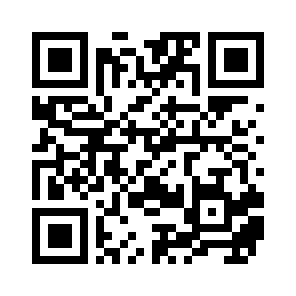
\includegraphics[width=4cm] {images/uncertified.png}
}

\author{Abdelrahman Abbas, Ahmed Elmenshawi, Nick Allison, Jimmy Bright}

\fancyhead[L]{Spi Users Guide}
\fancyhead[R]{\leftmark}
\fancyfoot[C]{Rocksavage Technology, Inc.~\copyright~2023}
\fancyfoot[R]{Page \thepage}

\begin{document}

\maketitle
\newpage
\tableofcontents

\section{Errata and Known Issues}

\subsection{Errata}
None.

\subsection{Known Issues}
None.

% chktex-file 44
\section{Port Descriptions}

\subsection{Spi Interface}

The ports for \textbf{Spi} are shown below in 
Table 1. The width of several ports is controlled 
by the following input parameters:

\renewcommand*{\arraystretch}{1.4}  % Adjust row height
 
\begingroup
\small
% \setlength{\arrayrulewidth}{1pt}
\rowcolors{2}{gray!30}{gray!10} % Alternating colors start from the second row
\arrayrulecolor{gray!80}

\begin{longtable}[H]{ 
  | p{0.20\textwidth}
  | p{0.20\textwidth}
  | p{0.12\textwidth}
  | p{0.43\textwidth} |
  }

\hline
\rowcolor{dark-gray}
\textcolor{white}{\textbf{Port Name}} & 
\textcolor{white}{\textbf{Width}} & 
\textcolor{white}{\textbf{Direction}} & 
\textcolor{white}{\textbf{Description}} \\ \hline
\endfirsthead

\hline
\rowcolor{dark-gray}
\textcolor{white}{\textbf{Port Name}} & 
\textcolor{white}{\textbf{Width}} & 
\textcolor{white}{\textbf{Direction}} & 
\textcolor{white}{\textbf{Description}}\\ \hline
\endhead

\hline
\endfoot

sclk &      
1 & 
Input/Output &     
Generated as Output by the Master to drive transactions to Slave. Taken as Input by Slave to respond to transactions\\ \hline

miso &       
1 & 
Input/Output &       
Input data for Master config. and Output data for Slave config. \\ \hline

mosi &        
1& 
Input/Output &       
Output data for Master config. and Input data for Slave config.\\ \hline

cs &      
1 & 
Input/Output &     
Driven as Output by Master to select Slave. Taken as Input by Slave to be activated\\ \hline


\end{longtable}
\captionsetup{aboveskip=0pt}
\captionof{table}{Spi Ports Descriptions}\label{table:ports}
\endgroup


\subsection{Apb3 Interface}
The \textbf{Apb3 Interface} is a regular Apb3 Slave Interface. All signals supported are shown below in 
Table 2. See the \textit{AMBA Apb Protocol Specifications} for a complete description of the signals. The width of several ports is controlled 
by the following input parameters:

\begin{itemize}[noitemsep]
  \item \textit{dataWidth} is the width of PWDATA and PRDATA in bits
  \item \textit{addrWidth} is the width of PADDR in bits
\end{itemize}
 
\renewcommand*{\arraystretch}{1.4}

\begingroup
\small
\rowcolors{2}{gray!30}{gray!10} % Alternating colors start from the second row
\begin{longtable}[H]{
  | p{0.20\textwidth}
  | p{0.20\textwidth}
  | p{0.12\textwidth}
  | p{0.43\textwidth} |
  }

  \hline
  \rowcolor{dark-gray}
  \textcolor{white}{\textbf{Port Name}} & 
  \textcolor{white}{\textbf{Width}} & 
  \textcolor{white}{\textbf{Direction}} & 
  \textcolor{white}{\textbf{Description}} \\ \hline
  \endfirsthead

  \hline
  \rowcolor{dark-gray}
  \textcolor{white}{\textbf{Port Name}} & 
  \textcolor{white}{\textbf{Width}} & 
  \textcolor{white}{\textbf{Direction}} & 
  \textcolor{white}{\textbf{Description}}\\ \hline
  \endhead

  \hline
  \endfoot


  PCLK &       
  1 &       
  Input &       
  Positive edge clock \\ \hline

  PRESETN &       
  1 &       
  Input &       
  Active low reset \\ \hline

  PSEL &       
  1 & 
  Input &       
  Indicates slave is selected and a data transfer is required \\ \hline

  PENABLE &        
  1 & 
  Input &       
  Indicates second cycle of Apb transfer \\ \hline

  PWRITE &        
  1 & 
  Input &       
  Indicates write access when HIGH and read access when LOW\\ \hline

  PADDR &      
  \textit{addrWidth} & 
  Input &     
  Address bus \\ \hline

  PWDATA &      
  \textit{dataWidth} & 
  Input &     
  Write data bus driven when PWRITE is HIGH\\ \hline

  PRDATA &      
  \textit{dataWidth} & 
  Output &     
  Read data bus driven when PWRITE is LOW\\ \hline
 
  PREADY &        
  1 & 
  Output &       
  Transfer ready \\ \hline

  PSLVERR &        
  1 & 
  Output &       
  Transfer error \\ \hline
  
\end{longtable}
\captionsetup{aboveskip=0pt}
\captionof{table}{Apb Ports Descriptions}\label{table:interface}
\endgroup

% chktex-file 44

\section{Parameter Descriptions}

The parameters for \textbf{Spi} are shown below in
Table 3.

\renewcommand*{\arraystretch}{1.4}
\begingroup
\small
\rowcolors{2}{gray!30}{gray!10} % Alternating colors start from the second row
\arrayrulecolor{gray!50}
\begin{longtable}[H]{
    | p{0.25\textwidth}
    | p{0.10\textwidth}
    | p{0.05\textwidth}
    | p{0.05\textwidth}
    | p{0.47\textwidth} |
  }
  \hline
  \rowcolor{dark-gray}

  \textcolor{white}{\textbf{Name}} &
  \textcolor{white}{\textbf{Type}} &
  \textcolor{white}{\textbf{Min}} &
  \textcolor{white}{\textbf{Max}} &
  \textcolor{white}{\textbf{Description}} \\ \hline
  \endfirsthead

  \textcolor{white}{\textbf{Name}} &
  \textcolor{white}{\textbf{Type}} &
  \textcolor{white}{\textbf{Min}} &
  \textcolor{white}{\textbf{Max}} &
  \textcolor{white}{\textbf{Description}}            \\ \hline
  \endhead


  \endfoot

  dataWidth   &
  Int       &
  1         &
  $\leq$ 32          &
  The data width of PWDATA, and PRDATA. Can be 8, 6, or 32 bits wide \\ \hline

  addrWidth     &
  Int           &
  1             &
  $\leq$ 32       &
  The Apb address bus width  \\ \hline

\end{longtable}
\captionsetup{aboveskip=0pt}
\captionof{table}{Parameter Descriptions}\label{table:params}
\endgroup

The Spi is instantiated into a design as follows:

\begin{lstlisting}[language=Scala]

  // Valid Spi Instantiation Example
  val mySpi = new Spi(
    dataWidth = 32, 
    addrWidth = 32 ) 

  \end{lstlisting}

\section{Operating Modes}
The SPI core's versatility is exemplified by its ability to operate in both master and slave modes. Each mode offers distinct functionalities and configurations to cater to diverse system requirements.

\subsection{Master Mode}
In master mode, the SPI core assumes control over the communication process. It is responsible for generating the serial clock (SCK) and managing the Slave Select (SS) lines to initiate and terminate communication with slave devices.

\subsubsection{Normal Mode}
Operating in normal mode without buffering involves the following characteristics:

\begin{itemize}
    \item \textbf{Immediate Transmission:} Data transmission begins as soon as data is written to the Data Register (\texttt{DATA}).
    \item \textbf{Single-Buffered Transmission:} The SPI core uses a single buffer for transmission, meaning only one byte can be sent at a time.
    \item \textbf{Double-Buffered Reception:} Reception is handled using a double buffer, allowing for more efficient data handling without data loss.
    \item \textbf{Write Collision Detection:} If an attempt is made to write to \texttt{DATA} before the current transmission completes, the Write Collision flag (\texttt{WRCOL}) is set, indicating a collision has occurred.
\end{itemize}

\subsubsection{Buffer Mode}
Enabling buffer mode introduces additional buffering capabilities, enhancing data handling efficiency:

\begin{itemize}
    \item \textbf{Double-Buffered Transmission:} Allows two bytes to be buffered for transmission, enabling continuous data flow without waiting for the previous transmission to complete.
    \item \textbf{Triple-Buffered Reception:} Reception is managed using three buffers, providing ample space to handle incoming data without overflow.
    \item \textbf{Interrupt-Driven Operations:} Buffer mode facilitates the use of interrupts for efficient data handling. The Data Register Empty Interrupt Flag (\texttt{DREIF}) can be used to determine when \texttt{DATA} is ready to accept new data.
    \item \textbf{Enhanced Throughput:} By allowing multiple bytes to be buffered, buffer mode significantly increases the data throughput, making it suitable for high-speed data transfers.
\end{itemize}

% Master Mode Timing Diagram
\begin{figure}[H]
    \centering
    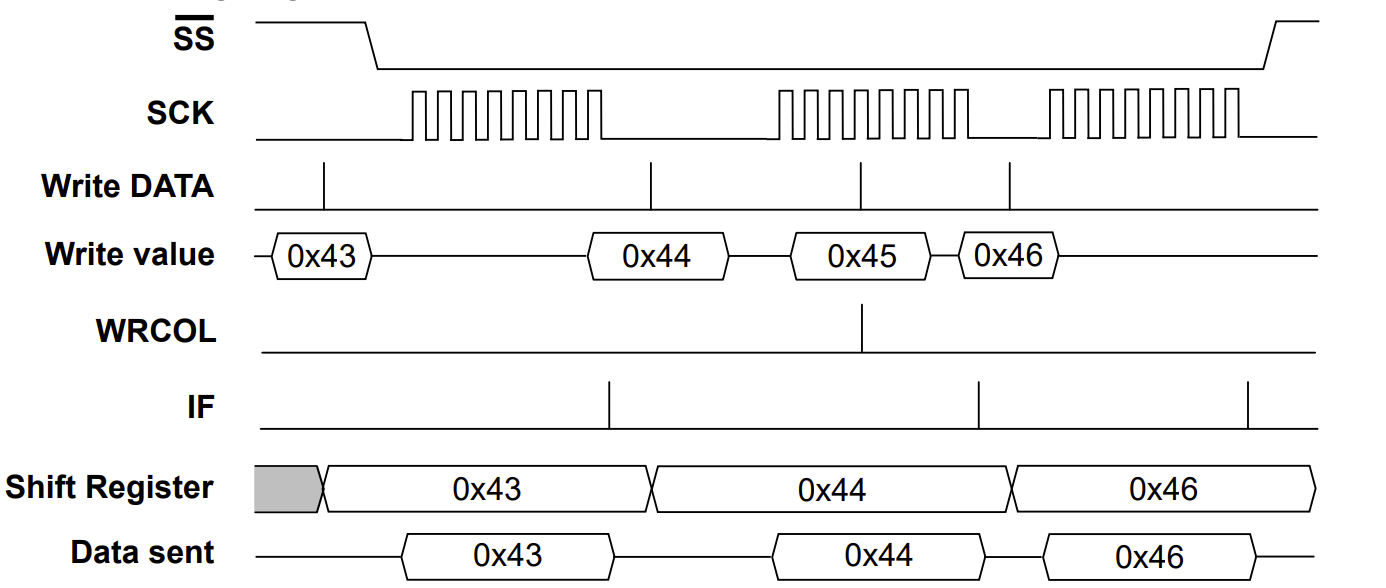
\includegraphics[width=0.85\textwidth]{images/spi_master_timing.png}
    \caption{Master Mode Timing Diagram}
    \label{fig:spi_master_timing}
\end{figure}

\subsubsection{Normal Mode}
In normal mode without buffering:

\begin{itemize}
    \item \textbf{Transmission starts immediately after writing to \texttt{DATA}.}
    \item \textbf{The core is single-buffered for transmission and double-buffered for reception.}
    \item \textbf{The Write Collision flag (\texttt{WRCOL}) is set if \texttt{DATA} is written before a transmission completes.}
\end{itemize}

\subsubsection{Buffer Mode}
Enabling buffer mode provides additional buffering:

\begin{itemize}
    \item \textbf{Double-buffered transmission and triple-buffered reception.}
    \item \textbf{Allows writing to \texttt{DATA} while a transmission is ongoing.}
    \item \textbf{Use the Data Register Empty Interrupt Flag (\texttt{DREIF}) to check if \texttt{DATA} can be written.}
\end{itemize}

% Buffer Mode Diagram
\begin{figure}[H]
    \centering
    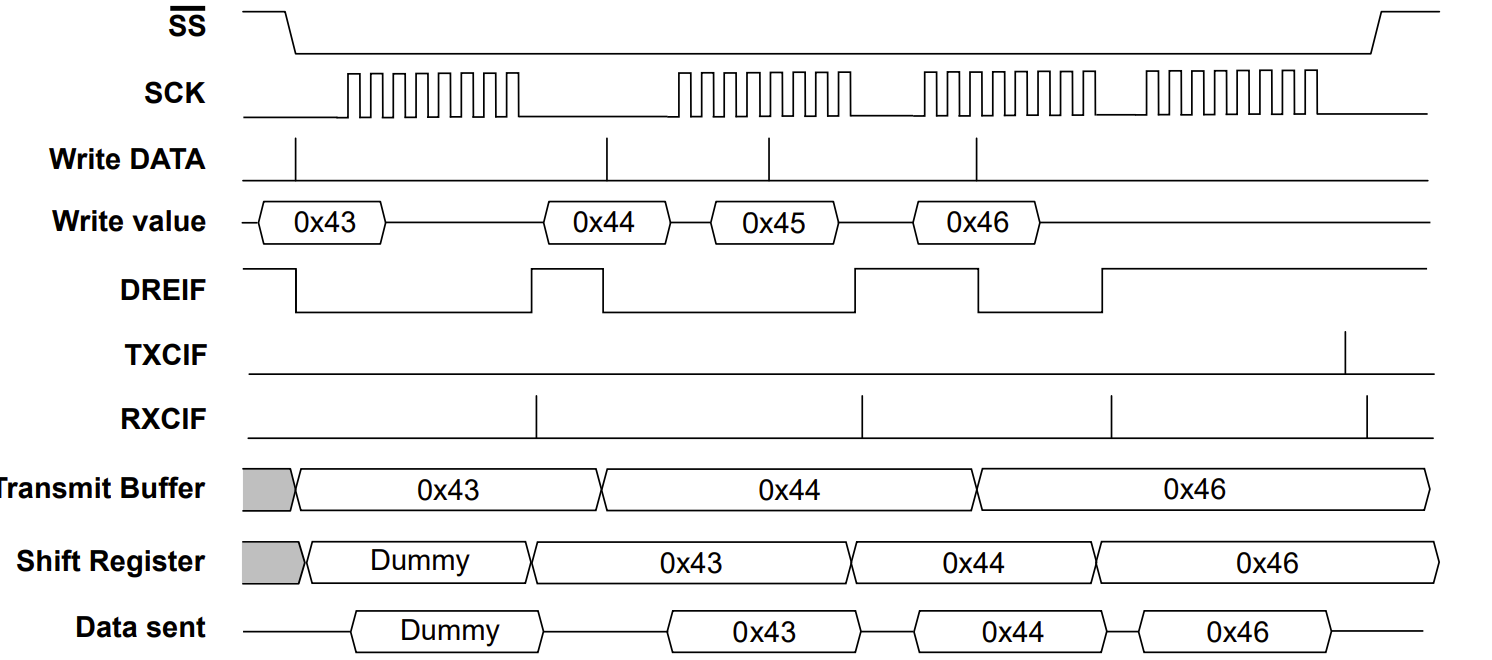
\includegraphics[width=0.85\textwidth]{images/spi_buffer_mode.png}
    \caption{SPI Buffer Mode Operation}
    \label{fig:spi_buffer_mode}
\end{figure}

\subsection{Slave Mode}
In slave mode, the SPI core operates passively, awaiting instructions from the master device. It does not generate the clock signal but instead responds to the master's SCK and SS signals.

\subsubsection{Normal Mode}
Operating in normal mode without buffering involves the following characteristics:

\begin{itemize}
    \item \textbf{Initiated by Master:} Transmission and reception are controlled by the master device, which dictates when data transfers occur.
    \item \textbf{Data Preparation:} Data must be written to the Data Register (\texttt{DATA}) before the master initiates a transfer. Failure to do so can result in incomplete or corrupted data transmission.
    \item \textbf{Write Collision Detection:} Similar to master mode, if \texttt{DATA} is written during an ongoing transfer, the Write Collision flag (\texttt{WRCOL}) is set, indicating a collision.
\end{itemize}

\subsubsection{Buffer Mode}
Buffer mode in slave operation offers enhanced data handling capabilities:

\begin{itemize}
    \item \textbf{Pre-Buffered Transmission:} Allows the slave to prepare multiple bytes of data in advance, ensuring seamless data transmission when the master initiates a transfer.
    \item \textbf{Graceful Overrun Handling:} Buffer mode can detect and manage data overruns, preventing data loss and maintaining system stability.
    \item \textbf{Configurable Buffer Behavior:} The Buffer Mode Wait for Receive (\texttt{BUFWR}) bit in \texttt{CTRLB} allows configuration of how the buffer behaves during data reception, enabling flexible data handling strategies.
\end{itemize}

% Slave Mode Timing Diagram
\begin{figure}[H]
    \centering
    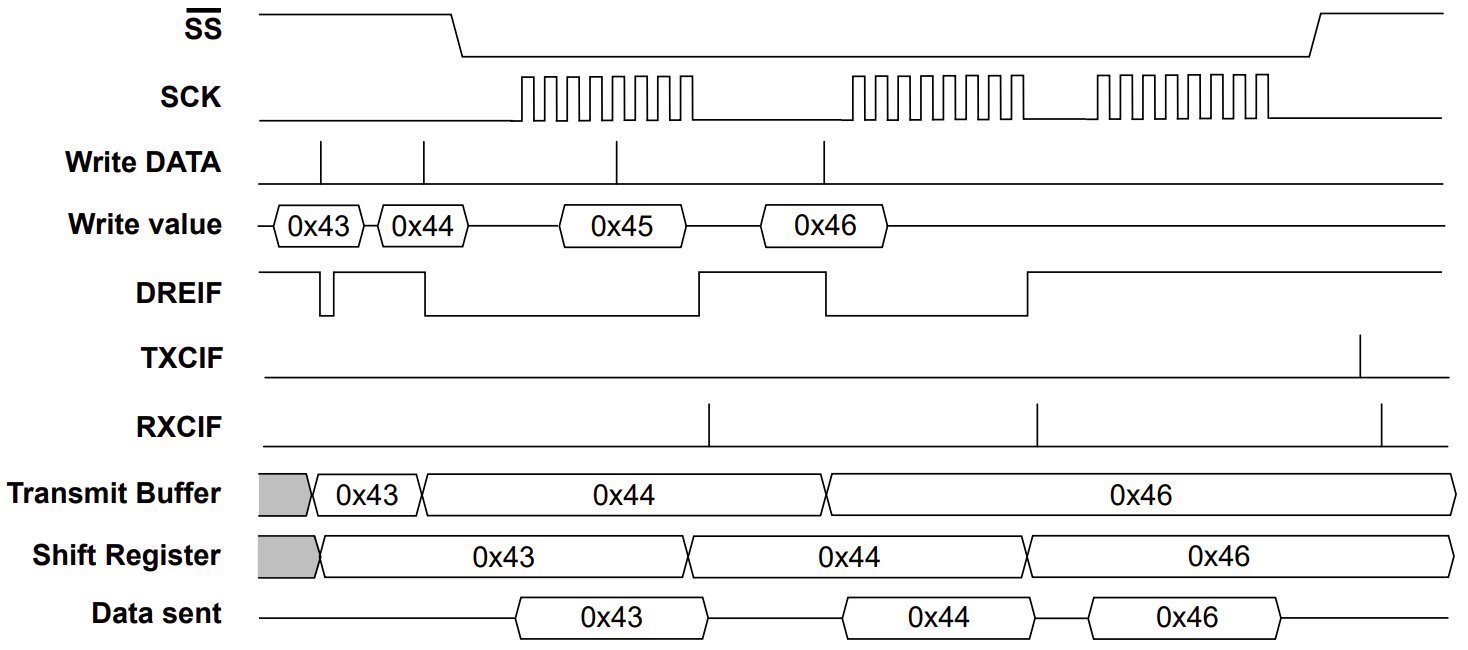
\includegraphics[width=0.85\textwidth]{images/spi_slave_timing.png}
    \caption{Slave Mode Timing Diagram}
    \label{fig:spi_slave_timing}
\end{figure}

\subsubsection{Normal Mode}
In normal mode:

\begin{itemize}
    \item \textbf{Transmission begins when SS is low and SCK pulses are received.}
    \item \textbf{Data must be written to \texttt{DATA} before the master initiates a transfer.}
    \item \textbf{The Write Collision flag (\texttt{WRCOL}) is set if \texttt{DATA} is written during an ongoing transfer.}
\end{itemize}

\subsubsection{Buffer Mode}
Buffer mode in slave operation allows for:

\begin{itemize}
    \item \textbf{Preparing data in advance for transmission.}
    \item \textbf{Handling data overruns more gracefully.}
    \item \textbf{Configurable behavior using the Buffer Mode Wait for Receive (\texttt{BUFWR}) bit.}
\end{itemize}

% % Slave Buffer Mode Diagram
% \begin{figure}[H]
%     \centering
%     \includegraphics[width=0.85\textwidth]{images/spi_slave_buffer_mode.png}
%     \caption{Slave Buffer Mode Operation}
%     \label{fig:spi_slave_buffer_mode}
% \end{figure}

\subsection{Data Transfer Modes}
The SPI protocol defines four distinct data transfer modes, each determined by the Clock Polarity (CPOL) and Clock Phase (CPHA). These modes dictate the timing relationship between the clock signal and data signals, ensuring synchronized and accurate data transmission.

\begin{table}[H]
    \centering
    \caption{SPI Data Transfer Modes}
    \begin{tabular}{@{}ccc@{}}
        \toprule
        \textbf{Mode} & \textbf{CPOL} & \textbf{CPHA} \\ \midrule
        0 & 0 & 0 \\
        1 & 0 & 1 \\
        2 & 1 & 0 \\
        3 & 1 & 1 \\ \bottomrule
    \end{tabular}
    \label{tab:spi_modes}
\end{table}

\begin{itemize}
    \item \textbf{Mode 0 (CPOL=0, CPHA=0):} 
    \begin{itemize}
        \item \textbf{Clock Polarity (CPOL):} The clock signal (SCK) is low when idle.
        \item \textbf{Clock Phase (CPHA):} Data is sampled on the leading (rising) edge of the clock.
        \item \textbf{Description:} Data is set up on the trailing edge and sampled on the leading edge, ensuring data stability before sampling.
    \end{itemize}
     
    \item \textbf{Mode 1 (CPOL=0, CPHA=1):}
    \begin{itemize}
        \item \textbf{Clock Polarity (CPOL):} The clock signal (SCK) is low when idle.
        \item \textbf{Clock Phase (CPHA):} Data is sampled on the trailing (falling) edge of the clock.
        \item \textbf{Description:} Data is set up on the leading edge and sampled on the trailing edge, providing flexibility in data timing.
    \end{itemize}
    
    \item \textbf{Mode 2 (CPOL=1, CPHA=0):}
    \begin{itemize}
        \item \textbf{Clock Polarity (CPOL):} The clock signal (SCK) is high when idle.
        \item \textbf{Clock Phase (CPHA):} Data is sampled on the leading (falling) edge of the clock.
        \item \textbf{Description:} Data is set up on the trailing edge and sampled on the leading edge, suitable for systems where a high idle clock state is preferred.
    \end{itemize}
    
    \item \textbf{Mode 3 (CPOL=1, CPHA=1):}
    \begin{itemize}
        \item \textbf{Clock Polarity (CPOL):} The clock signal (SCK) is high when idle.
        \item \textbf{Clock Phase (CPHA):} Data is sampled on the trailing (rising) edge of the clock.
        \item \textbf{Description:} Data is set up on the leading edge and sampled on the trailing edge, allowing for alternate data sampling strategies.
    \end{itemize}
\end{itemize}

% Data Transfer Modes Timing Diagrams
\begin{figure}[H]
    \centering
    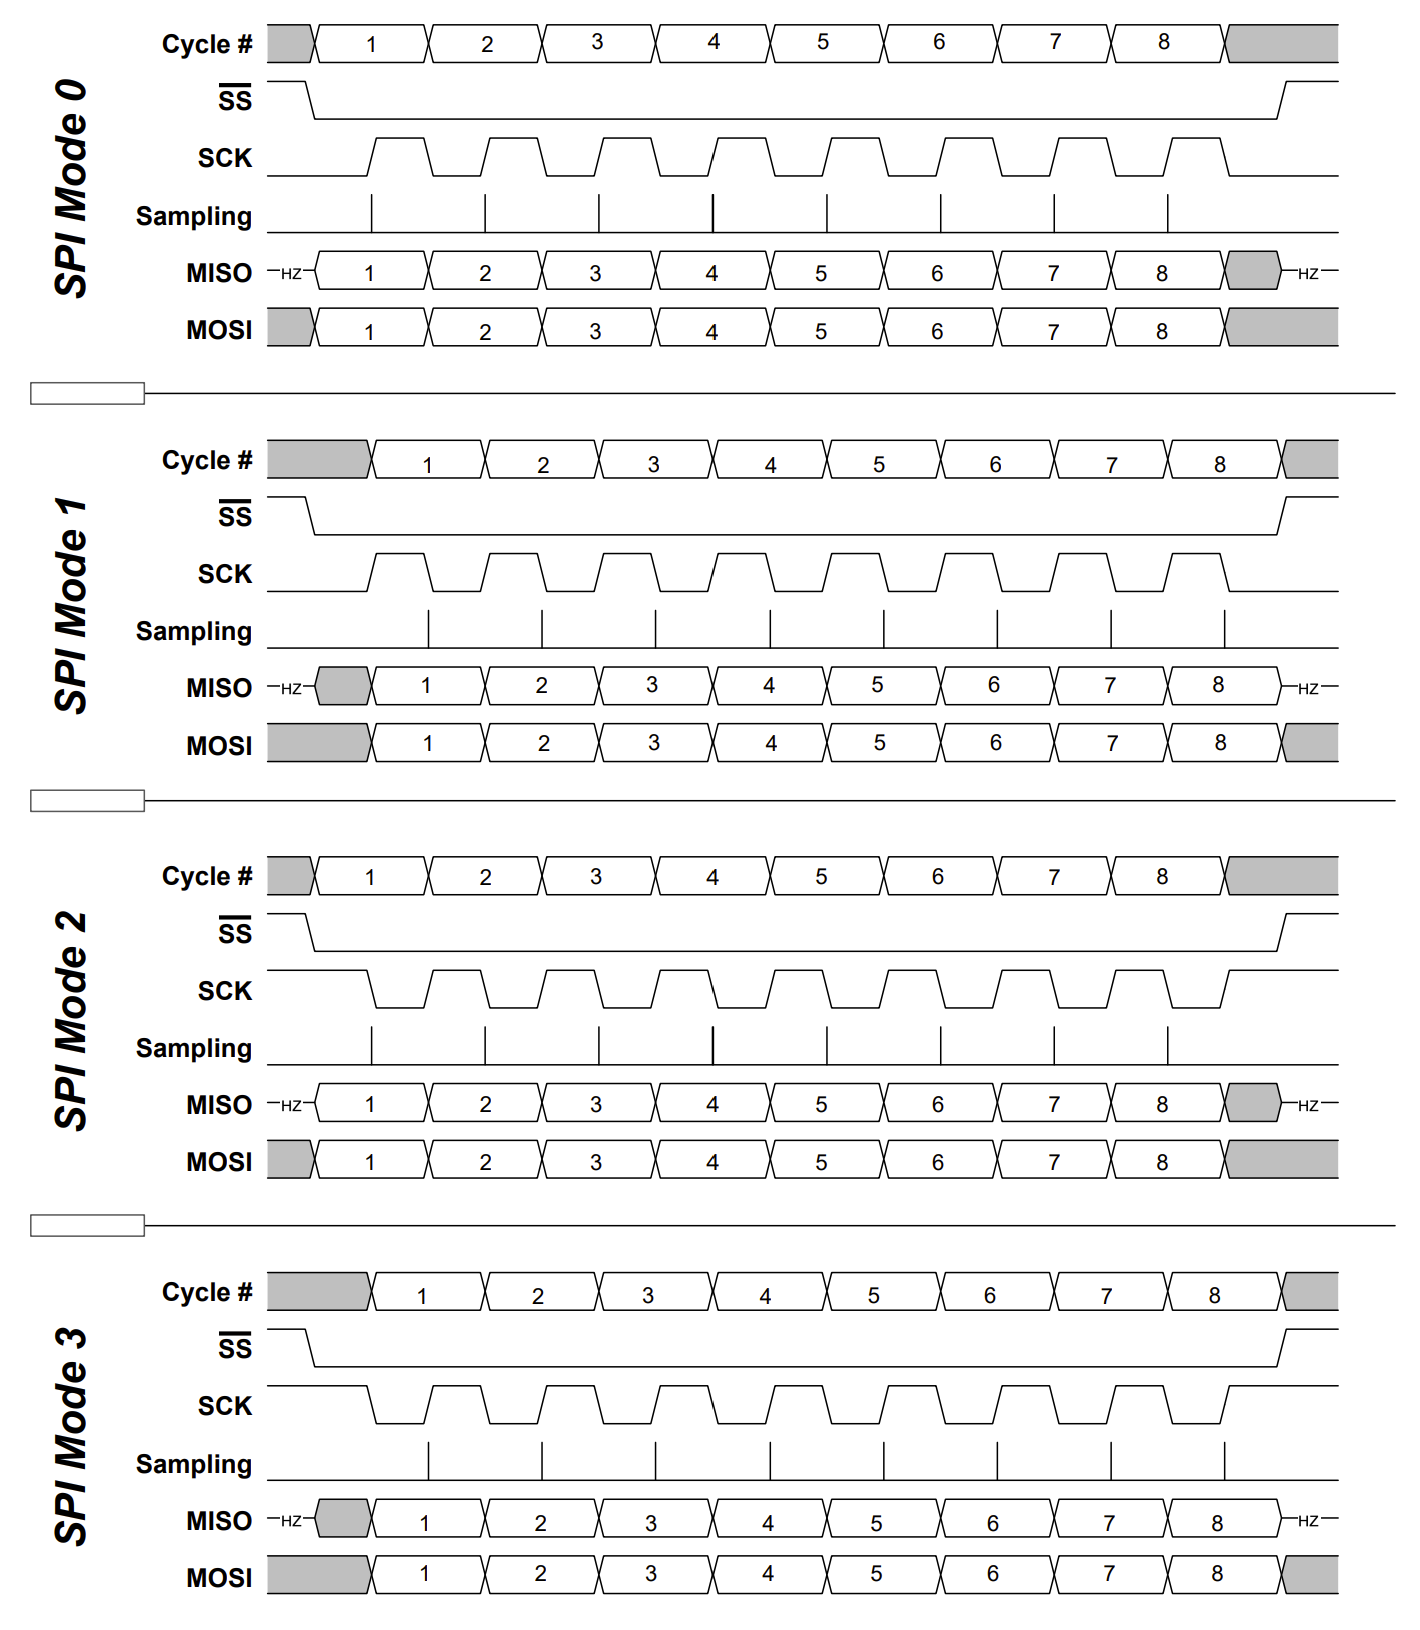
\includegraphics[width=0.9\textwidth]{images/spi_data_modes.png}
    \caption{SPI Data Transfer Modes Timing Diagrams}
    \label{fig:spi_data_modes}
\end{figure}

\section{Theory of Operations}

The SPI (Serial Peripheral Interface) core is equipped with a variety of features that make it a versatile and efficient choice for synchronous serial communication in embedded systems. These features
are described in-depth in the Register Interface section, but here is a brief overview:

\begin{itemize}
    \item \textbf{Full Duplex, Three-Wire Synchronous Data Transfer:} Enables simultaneous transmission and reception of data, enhancing communication efficiency.
    \item \textbf{Master or Slave Operation:} The SPI core can function as either a master, initiating and controlling communication, or as a slave, responding to the master's commands.
    \item \textbf{LSb First or MSb First Data Transfer:} Flexibly configures the data transmission order based on the system requirements, supporting both Least Significant Bit (LSb) first and Most Significant Bit (MSb) first formats.
    \item \textbf{Programmable Bit Rates:} Allows customization of the SPI clock speed to match the performance needs of different peripherals and system constraints.
    \item \textbf{End of Transmission Interrupt Flag:} Notifies the system when a data transmission cycle is complete, facilitating efficient interrupt-driven communication.
    \item \textbf{Write Collision Protection:} Prevents data corruption by detecting and handling scenarios where multiple write attempts occur simultaneously.
    \item \textbf{Wake-up from Idle Mode:} Supports low-power operations by enabling the SPI core to wake up from idle states upon specific events or triggers.
    \item \textbf{Double-Speed Master SPI Mode:} Increases data throughput by doubling the SPI clock rate in master mode, enhancing overall system performance.
\end{itemize}

% Block Diagram
\begin{figure}[H]
    \centering
    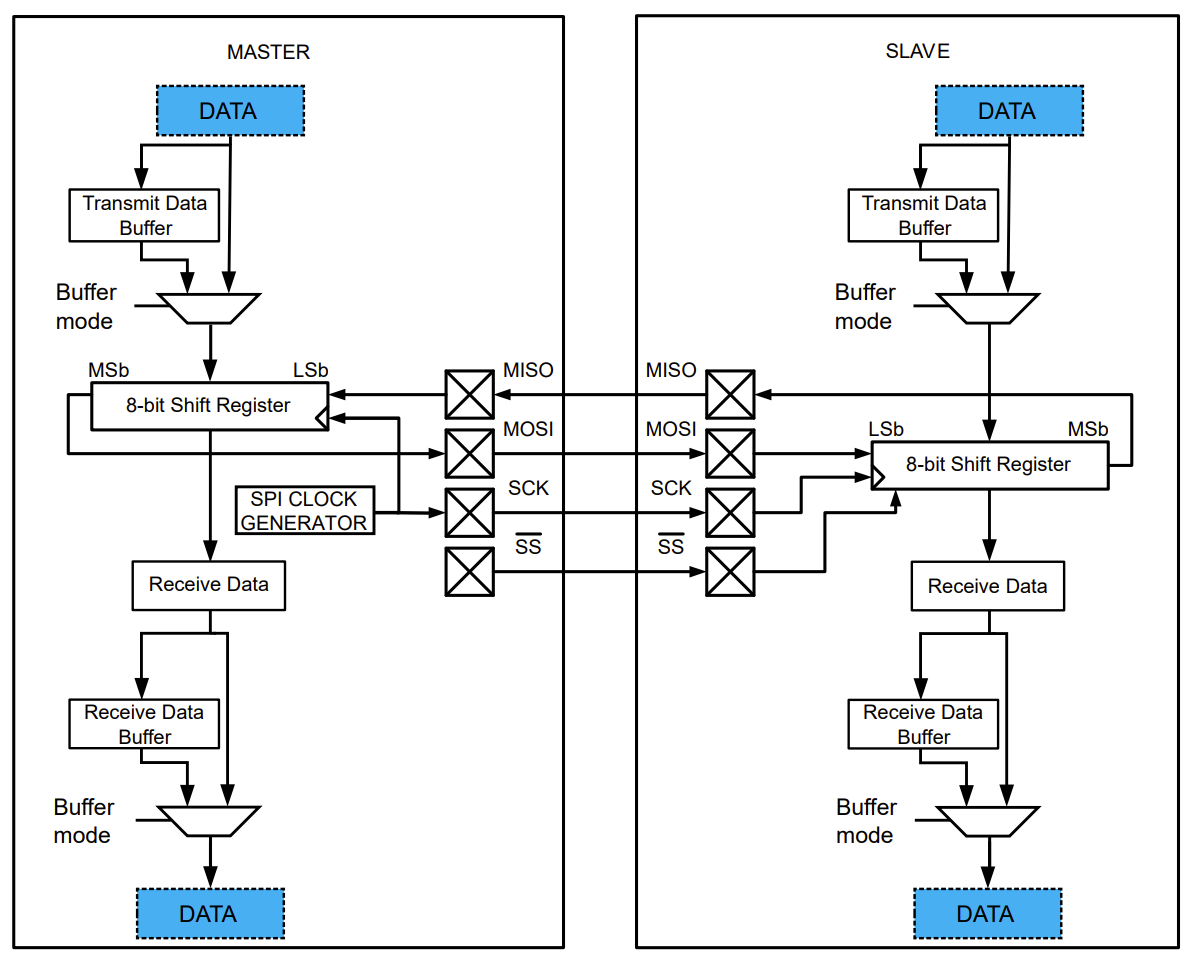
\includegraphics[width=0.8\textwidth]{images/spi_block_diagram.png}
    \caption{SPI Core Block Diagram}
    \label{fig:spi_block_diagram}
\end{figure}

\subsection{Interface Timing}

Spi has a synchronous Apb3 interface, and a Spi interface. The timing diagram shown below
in Figure~\ref{fig:timing} represents an instantiation with the following
parameters.

\begin{lstlisting}[language=Scala]
    val mySpi = new Spi(
      dataWidth = 8, 
      addrWidth = 8 ) 
\end{lstlisting}
    
\begin{figure}[h]
    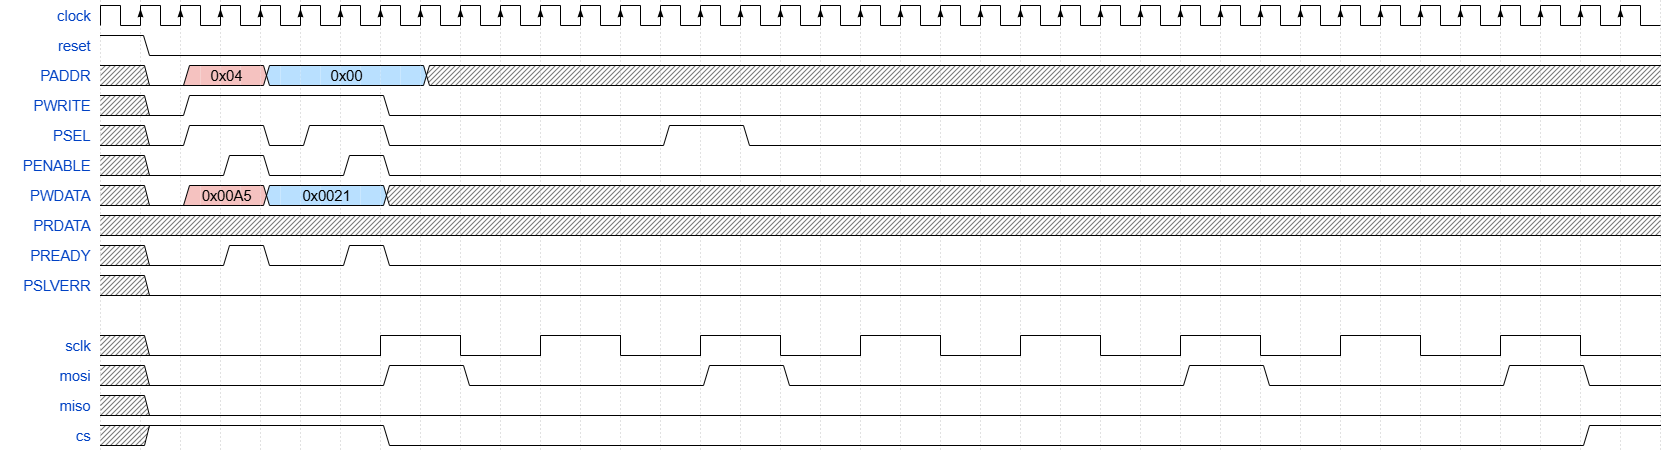
\includegraphics[width=\textwidth]{images/wavedrom.png}
    \caption{Timing Diagram}\label{fig:timing}
  \end{figure}

This shows the operation of enabling the Spi as a Master following the Apb protocol. Register CTRLA is written to configure the Master
as MSB first, prescaler set at 4, and no double clock speed. Since CTRLB is not written to, and its default values are 0, there will be no buffer mode, 
and CPOL/CPHA mode set to 0. The DATA register is written with 0xA5, which is the data the Master will transmit to the Slave. 

The \textit{sclk} port is driven once the master is enabled via CTRLA. Since CPOL/CPHA is set to 0, \textit{sclk} begins low, and sampling happens on the rising edge.
\textit{mosi} shifts out the value written to DATA, one bit at a time, MSB first. \textit{miso} stays low since the Slave is not sending any data to the Master. \textit{cs} 
is driven low once transmission begins, signalling to the Slave that a transaction is occuring.

Once the transaction is complete, all the SPI ports go low. 



% nested include
% chktex-file 44
\subsection{Register Interface}
 
When programming registers, each register starts on a byte address, and the last bits it would take up in its final byte based on its size are unused. To find the size in bytes for any register, divide by the register size, and round up to the nearest whole number. For example, a 32-bit register would take up 4 bytes, and a 1-bit register would take up 1 byte.
\renewcommand*{\arraystretch}{1.4}
\begingroup
\small
\rowcolors{2}{gray!30}{gray!10} % Alternating colors start from the second row
\arrayrulecolor{gray!50}
\begin{longtable}[H]{
  | p{0.27\textwidth}
  | p{0.18\textwidth}
  | p{0.50\textwidth} |
  }
  \hline
  \rowcolor{dark-gray}

  \textcolor{white}{\textbf{Name}} &   
  \textcolor{white}{\textbf{Size (Bits)}} &   
  \textcolor{white}{\textbf{Description}} \\ \hline \hline
  \endfirsthead

  \textcolor{white}{\textbf{Name}} &   
  \textcolor{white}{\textbf{Size (Bits)}} &   
  \textcolor{white}{\textbf{Description}} \\ \hline \hline
  \endhead

  
  CTRLA  &   
  8 &   
  Clock and Transmission Control Features \\ \hline

  CTRLB &   
  8 &   
  Transmission Mode Control \\ \hline

  INTCTRL &   
  8 &   
  Enable Flags for Interrupts \\ \hline

  INTFLAGS &   
  8 &   
  Interrupt Status Register \\ \hline

  DATA&   
  dataWidth &   
  Not a Physical Register. Connects to the shift register for transmitting and recieving. \\ \hline

\end{longtable}
\captionsetup{aboveskip=0pt}
\captionof{table}{Register Interface}\label{table:register}

  \newpage

  \subsection{Register Description}

  \subsection{Control Register A (\texttt{CTRLA})}
  \label{sec:ctrla}
  
  \begin{table}[H]
      \centering
      \caption{Control Register A (\texttt{CTRLA})}
      \begin{tabular}{@{}cccccccc@{}}
          \toprule
          \textbf{Bit} & 7 & 6 & 5 & 4 & 3 & 2-1 & 0 \\ \midrule
          \textbf{Name} & N/A & DORD & MASTER & CLK2X & N/A & PRESC[1:0] & ENABLE \\ \bottomrule
      \end{tabular}
      \label{tab:ctrl_a}
  \end{table}
  
  \begin{itemize}
      \item \textbf{Bit 6 - DORD (Data Order):} 
      \begin{itemize}
          \item \texttt{0}: MSB (Most Significant Bit) transmitted first.
          \item \texttt{1}: LSb (Least Significant Bit) transmitted first.
      \end{itemize}
      \textit{Description:} This bit configures the order in which data bits are transmitted and received. Selecting LSb first can be beneficial for certain peripherals or communication protocols that prioritize lower-order bits.
      
      \item \textbf{Bit 5 - MASTER:} 
      \begin{itemize}
          \item \texttt{0}: Slave mode.
          \item \texttt{1}: Master mode.
      \end{itemize}
      \textit{Description:} Determines whether the SPI core operates as a master or a slave. In master mode, the core generates the clock and controls SS lines. In slave mode, it responds to the master's commands.
      
      \item \textbf{Bit 4 - CLK2X (Clock Double):} 
      \begin{itemize}
          \item \texttt{0}: SPI clock rate not doubled.
          \item \texttt{1}: SPI clock rate doubled.
      \end{itemize}
      \textit{Description:} When set, this bit doubles the SPI clock frequency after prescaling in master mode, effectively increasing data transfer speed.
      
      \item \textbf{Bits 2-1 - PRESC[1:0] (Prescaler):} 
      \begin{itemize}
          \item \texttt{00}: Divide by 4.
          \item \texttt{01}: Divide by 16.
          \item \texttt{10}: Divide by 64.
          \item \texttt{11}: Divide by 128.
      \end{itemize}
      \textit{Description:} These bits define the base division factor applied to the peripheral clock to generate the SPI clock rate. Higher division factors result in lower SPI clock speeds.
      
      \item \textbf{Bit 0 - ENABLE:} 
      \begin{itemize}
          \item \texttt{0}: SPI disabled.
          \item \texttt{1}: SPI enabled.
      \end{itemize}
      \textit{Description:} Activates or deactivates the SPI core. Disabling the SPI core can save power when communication is not required.
  \end{itemize}
  
  \subsection{Control Register B (\texttt{CTRLB})}
  \label{sec:ctrlb}
  
  \begin{table}[H]
      \centering
      \caption{Control Register B (\texttt{CTRLB})}
      \begin{tabular}{@{}cccccccc@{}}
          \toprule
          \textbf{Bit} & 7 & 6 & 5 & 4 & 3-2 & 1-0 \\ \midrule
          \textbf{Name} & BUFEN & N/A & N/A & N/A & EIGHTB[3:2] & MODE[1:0] \\ \bottomrule
      \end{tabular}
      \label{tab:ctrl_b}
  \end{table}
  
  
  \begin{itemize}
      \item \textbf{Bit 7 - BUFEN (Buffer Enable):} 
      \begin{itemize}
          \item \texttt{0}: Buffer mode disabled.
          \item \texttt{1}: Buffer mode enabled.
      \end{itemize}
      \textit{Description:} When set, enables buffer mode, allowing the SPI core to handle multiple data bytes efficiently through additional buffering mechanisms.
      
      \item \textbf{Bits 3-2 - EIGHTB[3:2] (8 Bit Transactions):} 
      \begin{itemize}
          \item \texttt{00}: Data is not split into 8-bit transactions.
          \item \texttt{01}: Used for 16-bit configuration to split into 8-bit transactions.
          \item \texttt{10}: User for 32-bit configuration to split into 8-bit transactions.
          \item \texttt{11}: N/A.
      \end{itemize}
      \textit{Description:} Used to split 16-bit and 32-bit into 8-bit transactions. Note: Must be 00 for an 8-bit core.

      \item \textbf{Bits 1-0 - MODE[1:0] (Mode Selection):} 
      \begin{itemize}
          \item \texttt{00}: Mode 0.
          \item \texttt{01}: Mode 1.
          \item \texttt{10}: Mode 2.
          \item \texttt{11}: Mode 3.
      \end{itemize}
      \textit{Description:} Selects the SPI data transfer mode based on CPOL and CPHA settings, defining the timing relationship between the clock and data signals.
  \end{itemize}
  
  \subsection{Interrupt Control Register (\texttt{INTCTRL})}
  \label{sec:intctrl}
  
  \begin{table}[H]
      \centering
      \caption{Interrupt Control Register (\texttt{INTCTRL})}
      \begin{tabular}{@{}ccccccc@{}}
          \toprule
          \textbf{Bit} & 7 & 6 & 5 & 4 & 3-1 & 0 \\ \midrule
          \textbf{Name} & N/A & TXCIE & N/A & N/A & N/A & IE \\ \bottomrule
      \end{tabular}
      \label{tab:intctrl}
  \end{table}
  
  \begin{itemize}
      
      \item \textbf{Bit 6 - TXCIE (Transfer Complete Interrupt Enable):} 
      \begin{itemize}
          \item \texttt{0}: Transfer Complete interrupt disabled.
          \item \texttt{1}: Transfer Complete interrupt enabled.
      \end{itemize}
      \textit{Description:} Enables the generation of an interrupt when a data transmission cycle is complete in buffer mode, signaling that the transmit buffer is empty and ready for new data.
      
      \item \textbf{Bit 0 - IE (Interrupt Enable):} 
      \begin{itemize}
          \item \texttt{0}: General interrupts in normal mode disabled.
          \item \texttt{1}: General interrupts in normal mode enabled.
      \end{itemize}
      \textit{Description:} Controls the overall interrupt functionality in normal mode. When set, the SPI core can generate interrupts based on the \texttt{IF} flag in normal mode.
  \end{itemize}
  
  \subsection{Interrupt Flags Register (\texttt{INTFLAGS})}
  \label{sec:intflags}
  
  The Interrupt Flags Register (\texttt{INTFLAGS}) monitors various interrupt conditions and flags. Its behavior varies depending on whether the SPI core is operating in normal mode or buffer mode.
  
  \subsubsection{Normal Mode}
  In normal mode, the \texttt{INTFLAGS} register contains the following flags:
  
  \begin{table}[H]
      \centering
      \caption{Interrupt Flags Register (\texttt{INTFLAGS}) - Normal Mode}
      \begin{tabular}{@{}cc@{}}
          \toprule
          \textbf{Bit} & \textbf{Name} \\ \midrule
          7 & IF \\
          6 & WRCOL \\ \bottomrule
      \end{tabular}
      \label{tab:intflags_normal}
  \end{table}
  
  \begin{itemize}
      \item \textbf{Bit 7 - IF (Interrupt Flag):} 
      \begin{itemize}
          \item \texttt{0}: No interrupt.
          \item \texttt{1}: Interrupt flag set, indicating a data transfer has completed.
      \end{itemize}
      \textit{Description:} This flag is set automatically when a data transfer cycle is finished. It can be cleared by executing the corresponding interrupt vector or by reading the \texttt{INTFLAGS} register followed by accessing the \texttt{DATA} register.
      
      \item \textbf{Bit 6 - WRCOL (Write Collision Flag):} 
      \begin{itemize}
          \item \texttt{0}: No write collision detected.
          \item \texttt{1}: Write collision occurred, indicating an attempt to write to \texttt{DATA} during an ongoing transfer.
      \end{itemize}
      \textit{Description:} This flag alerts the system to potential data corruption caused by simultaneous write attempts. It must be cleared by first reading the \texttt{INTFLAGS} register and then accessing the \texttt{DATA} register.
  \end{itemize}
  
  \subsubsection{Buffer Mode}
  In buffer mode, the \texttt{INTFLAGS} register encompasses additional flags to manage enhanced data handling:
  
  \begin{table}[H]
      \centering
      \caption{Interrupt Flags Register (\texttt{INTFLAGS}) - Buffer Mode}
      \begin{tabular}{@{}cccccc@{}}
          \toprule
          \textbf{Bit} & 7 & 6 & 5 & 4 & 0 \\ \midrule
          \textbf{Name} & N/A & TXCIF & DREIF & N/A & BUFOVF \\ \bottomrule
      \end{tabular}
      \label{tab:intflags_buffer}
  \end{table}
  
  \begin{itemize}
      
      \item \textbf{Bit 6 - TXCIF (Transfer Complete Interrupt Flag):} 
      \begin{itemize}
          \item \texttt{0}: Transfer not complete.
          \item \texttt{1}: Transfer complete and transmit buffer is empty.
      \end{itemize}
      \textit{Description:} Signals that all data in the transmit shift register has been shifted out, and there is no new data pending in the transmit buffer. This flag is cleared by writing a \texttt{1} to its bit position.
      
      \item \textbf{Bit 5 - DREIF (Data Register Empty Interrupt Flag):} 
      \begin{itemize}
          \item \texttt{0}: \texttt{DATA} register is ready to accept new data.
          \item \texttt{1}: \texttt{DATA} register not ready for new data.
      \end{itemize}
      \textit{Description:} Indicates that the \texttt{DATA} register is empty and ready to receive new data for transmission. Writing new data to \texttt{DATA} clears this flag, either by writing the data or disabling the interrupt.
      
      \item \textbf{Bit 0 - BUFOVF (Buffer Overflow Flag):} 
      \begin{itemize}
          \item \texttt{0}: No buffer overflow.
          \item \texttt{1}: Buffer overflow detected.
      \end{itemize}
      \textit{Description:} Indicates that a buffer overflow has occurred during data reception, meaning the receive buffer was full when a new byte arrived. This flag is cleared by reading the \texttt{DATA} register or writing a \texttt{1} to its bit position.
  \end{itemize}
  
  \subsection{Data Register (\texttt{DATA})}
  \label{sec:data_register}
  The Data Register (\texttt{DATA}) serves as the primary interface for sending and receiving data through the SPI core.
  
  \begin{itemize}
      \item \textbf{Writing to \texttt{DATA}:}
      \begin{itemize}
          \item In \textbf{master mode}, writing a byte to \texttt{DATA} initiates the transmission process. The byte is shifted out via the MOSI line while simultaneously receiving data from the slave through the MISO line.
          \item In \textbf{slave mode}, writing to \texttt{DATA} prepares the data to be sent to the master during the next communication initiated by the master.
      \end{itemize}
      
      \item \textbf{Reading from \texttt{DATA}:}
      \begin{itemize}
          \item Reading from \texttt{DATA} retrieves the most recently received byte of data.
      \end{itemize}
      
      \item Note: DATA is not a physical register. Depending on what mode is configured, it is mapped to other registers as described below.

      \item \textbf{Behavior in Different Modes:}
      \begin{itemize}
          \item \textbf{Normal Mode:}
          \begin{itemize}
              \item \texttt{DATA} writes go directly to the shift register for immediate transmission.
              \item \texttt{DATA} reads fetch data from the Receive Data register.
          \end{itemize}
          \item \textbf{Buffer Mode:}
          \begin{itemize}
              \item \texttt{DATA} writes are stored in the Transmit Data Buffer register, allowing for buffered transmission.
              \item \texttt{DATA} reads retrieve data from the Receive Data Buffer register, ensuring that multiple received bytes can be handled efficiently.
          \end{itemize}
      \end{itemize}
  \end{itemize}
  
  \subsection{Register Addresses}
  
  \paragraph{dataWidth: 8}
  \begin{table}[H]
    \centering
    \begin{tabular}{|c|c|c|}
        \hline
        \rowcolor{darkgray}  % Dark grey background for header row
        \textcolor{white}{\textbf{Register Name}} & \textcolor{white}{\textbf{Address Start}} & \textcolor{white}{\textbf{Address End}} \\ \hline
        CTRLA & 0x0 & 0x0 \\ \hline
        CTRLB & 0x1 & 0x1 \\ \hline
        INTCTRL & 0x2 & 0x2 \\ \hline
        INTFLAGS & 0x3 & 0x3 \\ \hline
        DATA & 0x4 & 0x4 \\ \hline
    \end{tabular}
    \caption{8-bit Register Addressing}
  \end{table}
  
  \paragraph{dataWidth: 16}
  \begin{table}[H]
    \centering
    \begin{tabular}{|c|c|c|}
      \hline
      \rowcolor{darkgray}  % Dark grey background for header row
      \textcolor{white}{\textbf{Register Name}} & \textcolor{white}{\textbf{Address Start}} & \textcolor{white}{\textbf{Address End}} \\ \hline
      CTRLA & 0x0 & 0x0 \\ \hline
      CTRLB & 0x1 & 0x1 \\ \hline
      INTCTRL & 0x2 & 0x2 \\ \hline
      INTFLAGS & 0x3 & 0x3 \\ \hline
      DATA & 0x4 & 0x5 \\ \hline
    \end{tabular}
    \caption{16-bit Register Addressing}
  \end{table}
  
  \paragraph{dataWidth: 32}
  \begin{table}[H]
    \centering
    \begin{tabular}{|c|c|c|}
      \hline
      \rowcolor{darkgray}  % Dark grey background for header row
      \textcolor{white}{\textbf{Register Name}} & \textcolor{white}{\textbf{Address Start}} & \textcolor{white}{\textbf{Address End}} \\ \hline
      CTRLA & 0x0 & 0x0 \\ \hline
      CTRLB & 0x1 & 0x1 \\ \hline
      INTCTRL & 0x2 & 0x2 \\ \hline
      INTFLAGS & 0x3 & 0x3 \\ \hline
      DATA & 0x4 & 0x6 \\ \hline
    \end{tabular}
    \caption{32-bit Register Addressing}
  \end{table}
\include{./virtual}
\include{./atomic}

\section{Simulation}

\subsection{Tests}
The test bench generates a number (default is 50) configurations of the
DynamicFifo that are highly randomized. There are two flavors of tests:

\begin{itemize}
  \item {Directed tests that fill the FIFO with random data and then read back
        the results to verify that the read data matches the writted data.}
  \item {Lengthy random tests that are used to check odd combinations of
        configurations and to compile code coverage data.}
\end{itemize}

\subsection{Code coverage}
All inputs and outputs are checked to insure each toggle at least once. An error
will be thrown in case any port fails to toggle.

The only exception are the \emph{almostEmptyLevel} and \emph{almostFullLevel}
which are intended to be static during each simulation. These signals are
excluded from coverage checks.

\subsection{Running simulation}

Simulations can be run directly from the command prompt as follows:

\begin{verbatim}
  $ sbt "test"
\end{verbatim}

or from make as follows:

\texttt{\$ make test}

\subsection{Viewing the waveforms}

The simulation generates an FST file that can be viewed using a waveform viewer. The command to view the waveform is as follows:
\begin{verbatim}
  $ gtkwave ./out/test/Gpio.fst
\end{verbatim}

% chktex-file 44
\section{Synthesis}

\subsection{Area}

The Spi has been tested in a number of configurations and the following
results should be representative of what a user should see in their own
technology.

\renewcommand*{\arraystretch}{1.4}
\begingroup
\small
\begin{longtable}[H]{
    | p{0.15\textwidth}
    | p{0.15\textwidth}
    | p{0.17\textwidth}
    | p{0.20\textwidth}
    | p{0.15\textwidth} |
  }
  \hline
  \rowcolor{dark-gray}
  \textcolor{white}{\textbf{Config Name}}   &
  \textcolor{white}{\textbf{gpioWidth}}   &
  \textcolor{white}{\textbf{numVirtualPorts}}     &
  \textcolor{white}{\textbf{sizeOfVirtualPorts}}     &
  \textcolor{white}{\textbf{Gates}}           \\ \hline \hline
  \endfirsthead

  \textcolor{white}{\textbf{Config Name}}   &
    \textcolor{white}{\textbf{gpioWidth}}   &
    \textcolor{white}{\textbf{numVirtualPorts}}     &
    \textcolor{white}{\textbf{sizeOfVirtualPorts}}     &
    \textcolor{white}{\textbf{Gates}}           \\ \hline \hline
  \endhead

  \hline
  \endfoot

  8\_8\_8   &
  8                      &
  8                      &
  8                      &
  6734                   \\ \hline

  16\_8\_8  &
  16                     &
  8                      &
  8                      &
  9325                   \\ \hline

  32\_8\_8  &
  32                     &
  8                      &
  8                      &
  14981                  \\ \hline

\end{longtable}
\captionsetup{aboveskip=0pt}
\captionof{table}{Synthesis results}\label{table:area}
\endgroup

\subsection{SDC File}
An \texttt{.sdc} file is generated to provide synthesis and static timing
analysis tools guidance for synthesis.

The \texttt{Spi.sdc} file is emitted and found in the
\texttt{./out/sta} directory.

\subsection{Timing}

The following timing was extracted using the generated~.sdc files using the
Nangate 45nm free library.

\renewcommand*{\arraystretch}{1.4}
\begin{longtable}[H]{
    | p{0.20\textwidth}
    | p{0.08\textwidth}
    | p{0.12\textwidth}
    | p{0.13\textwidth}
    | p{0.15\textwidth}
    | p{0.15\textwidth} |
  }
  \hline
  \rowcolor{dark-gray}
  \textcolor{white}{\textbf{Config Name}}   &
  \textcolor{white}{\textbf{Period}}        &
  \textcolor{white}{\textbf{Duty Cycle}}    &
  \textcolor{white}{\textbf{Input Delay}}   &
  \textcolor{white}{\textbf{Output Delay}}  &
  \textcolor{white}{\textbf{Slack}}           \\ \hline \hline

  8\_8\_8     &
  5ns                    &
  50\%                   &
  20\%                   &
  20\%                   &
  1.79 (MET)               \\ \hline

  8\_8\_8  &
  5ns                    &
  50\%                   &
  20\%                   &
  20\%                   &
  1.79 (MET)               \\ \hline

  8\_8\_8  &
  5ns                    &
  50\%                   &
  20\%                   &
  20\%                   &
  1.81 (MET)               \\ \hline

  
\end{longtable}
\captionsetup{aboveskip=0pt}
\captionof{table}{Static Timing Analysis results}\label{table:timing}
\endgroup

\subsection{Multicycle Paths}
None.


\end{document}
